\documentclass[tikz]{standalone}
\usepackage{tikz}
\usepackage{amsmath,tikz}
\usetikzlibrary{
    shapes,
    shapes.geometric,
    shapes.symbols,
    shapes.arrows,
    shapes.multipart,
    shapes.callouts,
    shapes.misc,
    positioning}

\definecolor{purpleVue}{rgb}{0.6,0.5,0.9}

\definecolor{orangeVue}{rgb}{0.975,0.7,0.2}

\definecolor{greenVue}{rgb}{0.15,0.65,0.4}
\definecolor{redVue}{rgb}{0.95,0.45,0.55}
\begin{document}

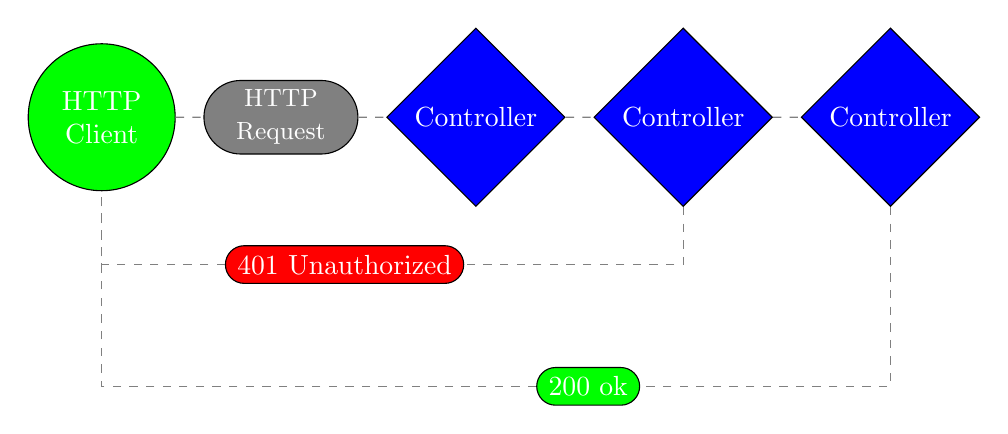
\begin{tikzpicture}
\node [draw, fill=green, text=white, circle, text width=4em, align=center] (client) {HTTP Client};
\node [draw, fill=gray, text=white, rounded rectangle, text width=4em, align=center, right=1em of client] (http) { \small{HTTP Request}};
\node[fill=blue, draw, shape=diamond, text=white, right=1em of http] (c1) {Controller};
\node[fill=blue, draw, shape=diamond, text=white, right=1em of c1] (c2) {Controller};
\node[fill=blue, draw, shape=diamond, text=white, right=1em of c2] (c3) {Controller};

% 401 response
\node[fill=red, draw, shape=rounded rectangle, text=white, below left=3em and -0.5em of c1] (401) {401 Unauthorized};
% 200 response
\node[fill=green, draw, shape=rounded rectangle, text=white, below right=3em and 4em of 401] (200) {200 ok};
% Paths last

\path[draw,dashed, color=gray] (client) -- (http) -- (c1) -- (c2) -- (c3);

\path[draw, dashed, color=gray] (c2) |- (401) (401) -| (client);

\path[draw, dashed, color=gray] (c3) |- (200) (200) -| (client);
\end{tikzpicture}

\end{document}
